\section{Data association}

The data association problem Revolve NTNU faces when making a driverless car for Formula Student differs in a few ways from the problems solved in the literature. The difference lies in that it is possible to add more restraints to the problem. The positions of the landmarks are quite regular, the rules stating that it should never be more than \SI{5}{\meter} between consecutive cones on either side, and the track width is never less than \SI{3}{\meter}. The cones are not too close either. The latter property is not stated explicitly in the rules, but is seen by looking at the videos of the events from previous years, and by talking with alumni that attended the competitions. 

The problem is also simplified by looking at data from the detection algorithms. First of all the false positives that arrive are not randomly positioned, but rather stem from objects or walls in the vicinity of the track that are not cones. This means they all lie outside of the track and therefore are not too dangerous if they enter into the map. 

Secondly the false positives that come from walls or large objects are not constant in position. This is taken advantage of by having new possible landmarks need more than one verification before being accepted, and every time a hypothesis does not get a new association its confidence is decreased. This means that a wall will spawn new landmarks along it that then decay in confidence and eventually get discarded, as long as we are not unlucky and get enough measurements to almost the same spot. Data from last year shows that this is not a problem. 

Lastly it is possible to take advantage of the fact that the different detection algorithms have different false positive rates. The camera for example barely ever accepts a false positive, but has a rather large error in the position of the detected cone. This is also used to our benefit, as will be explained below. 

All these simplifications lead us to believe that a compatibility test based approach would be beneficial. It would allow to take full advantage of the structure of the track, while avoiding the large computational cost of approaches like \gls{JPDA}.

\subsection{Summary of data association design}

The overall ideas of the data association scheme developed in this thesis is illustrated in figure \ref{Fig:FrontendDesign}. 

\begin{figure}
    \centering
    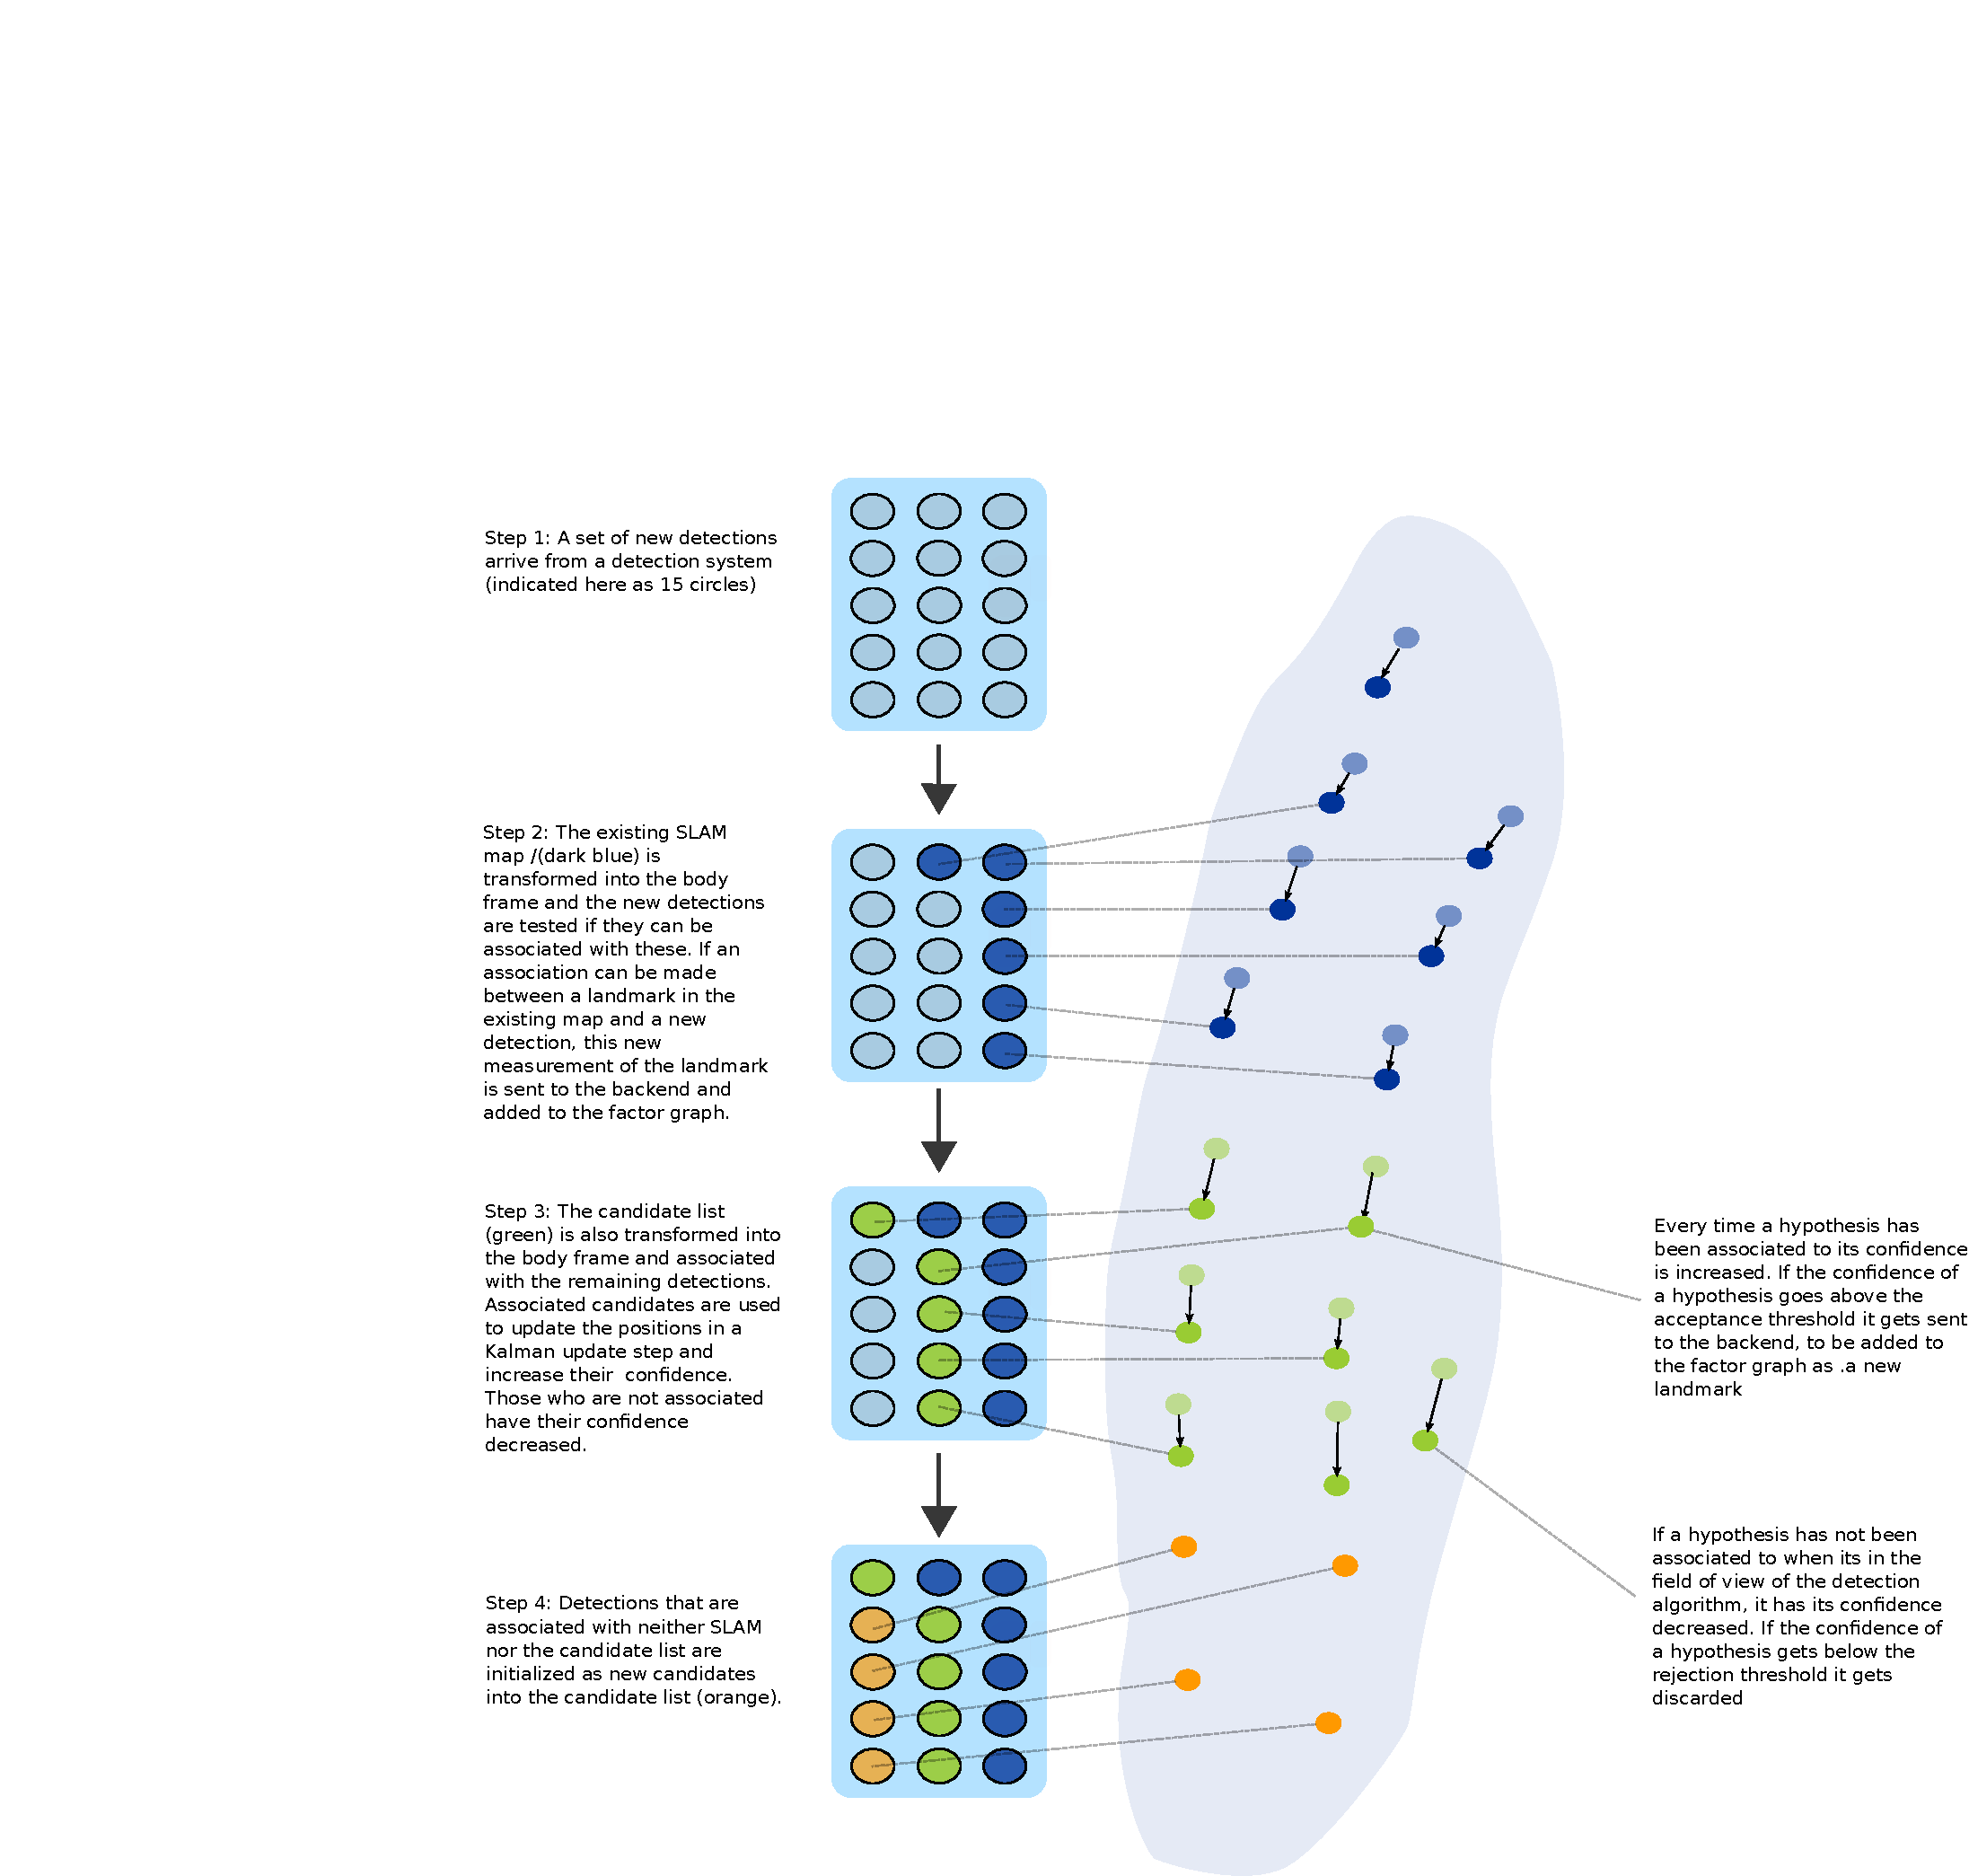
\includegraphics[width=\linewidth]{0_Images/3_Theory/sensor_fuser.pdf}
    \caption[Illustration of the main ideas of the data association scheme.]{Illustration of the main ideas of the data association scheme. How a new set of detections are compared with the map and then the hypothesis list before finally any remaining detections are initialised as new hypotheses.}
    \label{Fig:FrontendDesign}
\end{figure}

\todo[inline]{Fix missing dot in FrontendDesign figure.}

The chosen design uses ideas from the \gls{PDA} and compatibility test methods, while simplifying a bit because of the inherent limitations of the specific problem being solved. The main idea is as follows:

When a new set of detections arrive, they are compared with the latest map coming out of \gls{SLAM} using a compatibility test to associate new measurements with existing landmarks. Any positive associations are sent to the \gls{SLAM} backend to be added to the graph as new measurements of existing landmarks.

The measurements that can not be associated to the map are then compared with a list of hypotheses, using the same compatibility test. A hypothesis that gets a new measurement associated to it gets its confidence increased, while the ones that do not get their confidence decreased. The measurements that could not get associated to neither the map nor the list of hypotheses gets added to the list of hypotheses. 

\subsection{Comparison with the existing map}

Each measurement coming out of the detection algorithms has a covariance matrix that represents the uncertainty in both the detection systems position estimate and the estimate of the relative pose between the sensor and the body frame.

This means that when a set of new measurements arrive at the \gls{SLAM} frontend they consist of a vector of measurements and their covariance matrices. The covariance matrices, $\Sigma_{r,\psi}$, are aligned with the radial and yaw directions of the local polar coordinate frame that sits on top of each cone. These are then rotated into the body frame using the following formula

\begin{equation}
    \Sigma_{body} = R^T(\alpha)\Sigma_{r,\psi}R(\alpha)
    \label{DetectToBodyRot}
\end{equation}

where 

\begin{equation}
    R(\alpha) = \begin{bmatrix} cos(\alpha) & -sin(\alpha) \\ sin(\alpha) & cos(\alpha)
    \end{bmatrix}
\end{equation} 

and $\alpha$ is the angle between the x-axis of the body frame and the line between \gls{CG} and the cone in question. 

\begin{figure}
    \centering
    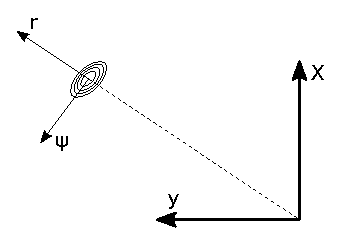
\includegraphics[width=0.5\linewidth]{0_Images/3_Theory/DetectionFrame.eps}
    \caption[The Gaussian distribution of each detected cone.]{The Gaussian distribution of each detected cone, shown with the body frame and height curves of the Gaussian noise on the detected cones position.}
    \label{Fig:DetectionFrame}
\end{figure}

Each detected cone is then transformed into the map frame, using the latest estimate of the car's position coming from the odometry, as well as the correction on the odometry that \gls{SLAM} outputs. Since the last time a detection arrived, the odometry covariance has been accumulated and is now added to all the landmarks in the map. 

This accumulation is simply summing of the diagonal covariance matrices of each odometry message, i.e. the covariance in the change of $x$, $y$ and $\psi$. This information arrives as covariances in the body frame, and even though this body frame will rotate and translate with respect to the map frame, it is assumed to never be a long time between the arrival of each set of detections. Therefore it is assumed that the step from the last detection can be approximated as a single translation followed by a single rotation. This assumption is used to simplify the process of summing the covariances. 

Instead of integrating the covariance along the trajectory of the car, the covariance in $x$ and $y$ of the accumulated odometry is simply summed and rotated into the global frame before getting added to the covariance of each landmark in the map. This is of course a simplification, but it avoids having to iterate through the map each time a new odometry message arrives, which is at $\SI{400}{Hz}$, thus leading to a lot of unnecessary computation. The team believes this error will be dominated by errors in the covariance estimates, so computation time was chosen over accuracy. 

The yaw covariance is accumulated by summation as well, but increases the covariance of each landmark in a different manner. The covariance in yaw of the accumulated step will lead to an increased covariance of each landmark that is approximately aligned with the $\psi$-direction in the local polar coordinate frame that sits on top of each landmark. The magnitude of this covariance is the accumulated covariance, $\sigma_{\psi}^2$, $r$, between the landmark and the car. This leads to a covariance matrix aligned with the local polar coordinate frame, which is then rotated into the body frame and added to the covariance of the landmark

\begin{equation}
    \Sigma^{new} = \Sigma^{old} + R(\alpha)diag\{0,\sigma^2_{\psi}\}
\end{equation}

Here $\Sigma^{old}$ is the old covariance of the landmark, $\Sigma^{new}$ is the new and $R(\alpha)$ is the rotation matrix aligning the local polar coordinate frame with the body frame, defined in equation \ref{DetectToBodyRot}. 

The closest landmark in the map to each cone is then found, and a compatibility test is done for each detected cone, using the covariance of the detected cone and the covariance of the closest landmark. All positive associations are then sent to SLAM as new measurements to existing landmarks. This information also includes the pose the car was in when it saw the landmarks. 

Since the race track follows some strict rules regarding spacing between landmarks, there will never be  cones too close together. Therefore each landmark has a safety zone around it of about 1 \si{\metre}. If a detection is within the safety radius of an already existing landmark, but does not pass the compatibility test with it, it gets discarded. This rule might mean discarding the few cones where this is not true, but it also makes the system overall more robust to outliers, so the team believes the trade off is worth it.  All the remaining detections are kept for comparison with the set of hypotheses. 

\subsection{Comparison with the set of hypotheses}

In the next step, the remaining detections are compared with the list of hypotheses. This is done the same way as for comparing with the map, by increasing the spatial covariance of all hypotheses, and association through a simple compatibility test, where the Mahalanobis distance must be below a threshold. One major difference is however that if two detections from the same detection algorithm at the same time step can be associated to the same hypotheses, then both the measurements and the hypotheses are discarded as outliers. This simplification means no care must be taken with overlapping hypotheses, like what is done in the \gls{JPDA}. 

\subsubsection{Positive associations}

A positive association with a hypothesis means that the confidence of this hypothesis is increased, and the measurement is added to the list of measurements of this hypothesis. How much the confidence is increased was initially going to be a function of distance from the car, but the ratio between the number of false and true positives have so far not turned out to be dependent on distance or angle in any meaningful way. For now the initial confidence is therefore just a function of which detection system the measurement came from. This is because there are fewer false positives from the camera algorithm than from the two \gls{LiDAR} systems. 

A positive association also means that the position estimate of the hypothesis is updated by a Kalman update step. This is done by first finding the distance between the measured position $z_{k-1}$ and the estimated one, $\hat{x}_{k|k-1}$. Call this distance $\Tilde{x}_k$. To find the optimal weighting between the new measurement and the previous estimate, the so called Kalman gain, $K_k$, is created

\begin{equation}
    K_k = P_{k|k-1}S^{-1}_k
\end{equation}

where $S_k$ is defined as 

\begin{equation}
    S_k = R_k + P_{k|k-1}
\end{equation}

Here, $R_k$ is the measurement noise and $P_{k|k-1}$ is the covariance of the landmark. This gain is then used to give a high weight to the measurement when the measurement noise is low and system noise is high, and vice versa. The new estimated position of the landmark is then

\begin{equation}
    \hat{x}_{k|k} = \hat{x}_{k|k-1} + K_k\Tilde{y}_k
\end{equation}

The keen reader might notice that there is no $H_k$ in the above equation. This is because our measurement function is the identity. 

The new covariance, $P_{k|k}$, of the landmark is then found by  

\begin{equation}
    P_{k|k} = (I-K)(P_{k|k-1} + Q)
\end{equation}

This shrinks the covariance if the measurement and previous estimate are close together, and increase it if they are far apart. In reality the covariance will always get smaller when a measurement is associated to a hypothesis, because of the compatibility test. 

\subsubsection{Lack of association}

If a hypothesis is not associated to when a new set of detections arrive, its confidence is decreased. How much it is decreased by is a function of which detection system this set of detections came from, and whether or not this hypothesis is in the field of view of the detection system. 

\subsubsection{Belief correction}

When a hypothesis' confidence climbs above a threshold it is accepted as an inlier and all the measurements of it are sent to SLAM as measurements of a new landmark. Similarly when the confidence goes below a threshold it is discarded. A hypothesis is also discarded when its spatial covariance gets too large. This is because we do not want ambiguity when associating measurements to hypotheses. 

The remaining measurements are then initialised as a new hypothesis. It is given an initial confidence that is a function of detection method.


\subsection{Loop closure}

The detection systems are capable of recognising the large orange cones that represent the start of the track. The start of the track has two of these orange cones on each side. 

This information is very valuable for \gls{SLAM}, as it represent what is called a loop closure. Loop closing is the task of deciding whether or not a vehicle has, after an excursion of arbitrary length, returned to a previously visited area.  

To incorporate this information into the graph the frontend waits until more than one orange cone is seen at the same time. The cones must also be closer than 1 \si{\metre}, as it is not desired to close the loop when the orange cones are seen far away. When these criteria are fulfilled, a connection between the current pose and the initial pose is added to the \gls{SLAM} graph. Since it is highly unlikely that the car is in the exact same spot, the connection between these poses is initialised with a rather large uncertainty.